\documentclass{book}
\usepackage[a4paper,top=2.5cm,bottom=2.5cm,left=2.5cm,right=2.5cm]{geometry}
\usepackage{makeidx}
\usepackage{natbib}
\usepackage{graphicx}
\usepackage{multicol}
\usepackage{float}
\usepackage{listings}
\usepackage{color}
\usepackage{ifthen}
\usepackage[table]{xcolor}
\usepackage{textcomp}
\usepackage{alltt}
\usepackage{ifpdf}
\ifpdf
\usepackage[pdftex,
            pagebackref=true,
            colorlinks=true,
            linkcolor=blue,
            unicode
           ]{hyperref}
\else
\usepackage[ps2pdf,
            pagebackref=true,
            colorlinks=true,
            linkcolor=blue,
            unicode
           ]{hyperref}
\usepackage{pspicture}
\fi
\usepackage[utf8]{inputenc}
\usepackage{mathptmx}
\usepackage[scaled=.90]{helvet}
\usepackage{courier}
\usepackage{sectsty}
\usepackage{amssymb}
\usepackage[titles]{tocloft}
\usepackage{doxygen}
\lstset{language=C++,inputencoding=utf8,basicstyle=\footnotesize,breaklines=true,breakatwhitespace=true,tabsize=4,numbers=left }
\makeindex
\setcounter{tocdepth}{3}
\renewcommand{\footrulewidth}{0.4pt}
\renewcommand{\familydefault}{\sfdefault}
\hfuzz=15pt
\setlength{\emergencystretch}{15pt}
\hbadness=750
\tolerance=750
\begin{document}
\hypersetup{pageanchor=false,citecolor=blue}
\begin{titlepage}
\vspace*{7cm}
\begin{center}
{\Large Pumpki\-Nibble }\\
\vspace*{1cm}
{\large Generated by Doxygen 1.8.2}\\
\vspace*{0.5cm}
{\small Sun Dec 2 2012 00:13:54}\\
\end{center}
\end{titlepage}
\clearemptydoublepage
\pagenumbering{roman}
\tableofcontents
\clearemptydoublepage
\pagenumbering{arabic}
\hypersetup{pageanchor=true,citecolor=blue}
\chapter{license}
\label{md_license}
\hypertarget{md_license}{}
M\-O\-D\-I\-F\-I\-E\-D D\-O W\-H\-A\-T T\-H\-E F\-U\-C\-K Y\-O\-U W\-A\-N\-T T\-O P\-U\-B\-L\-I\-C L\-I\-C\-E\-N\-S\-E Version 1, August 2012 Based on W\-T\-F\-P\-L version 2

Original W\-T\-F\-P\-L Copyright (C) 2004 Sam Hocevar \href{mailto:sam@hocevar.net}{\tt sam@hocevar.\-net} Copyright (C) 2012 ron975 Everyone is permitted to copy and distribute verbatim or modified copies of this license document, and changing it is allowed

D\-O W\-H\-A\-T T\-H\-E F\-U\-C\-K Y\-O\-U W\-A\-N\-T T\-O P\-U\-B\-L\-I\-C L\-I\-C\-E\-N\-S\-E T\-E\-R\-M\-S A\-N\-D C\-O\-N\-D\-I\-T\-I\-O\-N\-S F\-O\-R C\-O\-P\-Y\-I\-N\-G, D\-I\-S\-T\-R\-I\-B\-U\-T\-I\-O\-N A\-N\-D M\-O\-D\-I\-F\-I\-C\-A\-T\-I\-O\-N 0. The source code of all derivative works must be available to the public
\begin{DoxyEnumerate}
\item The source code of all derivative works must be available under this license
\item You are free to do whatever the fuck you want to with the source as long as you do not violate terms 0. and 1. 
\end{DoxyEnumerate}
\chapter{Pumpki\-Nibble}
\label{md_readme}
\hypertarget{md_readme}{}
Pumpki\-Nibble lets you and your players eat Pumpkin Seeds and more in Minecraft. Everything is configurable!

\section*{Compiling}

Check out this repository, then do '''mvn install pumpkinibble''' An installation of Maven 2 or higher is required

\section*{Development Builds}

Pumpki\-Nibble uses Maven and Build\-Hive to handle automatic builds You can download the latest builds from \href{https://buildhive.cloudbees.com/job/ron975/job/PumpkiNibble}{\tt https\-://buildhive.\-cloudbees.\-com/job/ron975/job/\-Pumpki\-Nibble}

\section*{Migrating from version 0.\-1}

Since Pumpki\-Nibble 1.\-0, Pumpki\-Nibble uses a completely different configuration file. You will need to remove and redo your configuration.

See more at \href{http://dev.bukkit.org/server-mods/pumpkinibble/}{\tt http\-://dev.\-bukkit.\-org/server-\/mods/pumpkinibble/} 
\chapter{Deprecated List}
\label{deprecated}
\hypertarget{deprecated}{}

\begin{DoxyRefList}
\item[\label{deprecated__deprecated000002}%
\hypertarget{deprecated__deprecated000002}{}%
Member \hyperlink{classnet_1_1mystia_1_1_pumpki_nibble_1_1_pumpki_nibble_a_p_i_a6e0a09ba0c5dfbcd859b955106d6d443}{net.mystia.Pumpki\-Nibble.Pumpki\-Nibble\-A\-P\-I.get\-Valid\-Items\-As\-String} (String separator)]Does not use String\-Buffer nor is required  
\item[\label{deprecated__deprecated000001}%
\hypertarget{deprecated__deprecated000001}{}%
Member \hyperlink{classnet_1_1mystia_1_1_pumpki_nibble_1_1_pumpki_nibble_a_p_i_a83f91739357b5326fdd35e3cf8f1f007}{net.mystia.Pumpki\-Nibble.Pumpki\-Nibble\-A\-P\-I.get\-Valid\-Types} ()]Is not required for plugin usage 
\end{DoxyRefList}
\chapter{Hierarchical Index}
\section{Class Hierarchy}
This inheritance list is sorted roughly, but not completely, alphabetically\-:\begin{DoxyCompactList}
\item \contentsline{section}{net.\-mystia.\-Pumpki\-Nibble.\-Pumpki\-Nibble\-A\-P\-I}{\pageref{classnet_1_1mystia_1_1_pumpki_nibble_1_1_pumpki_nibble_a_p_i}}{}
\item Command\-Executor\begin{DoxyCompactList}
\item \contentsline{section}{net.\-mystia.\-Pumpki\-Nibble.\-Pumpki\-Nibble\-Command}{\pageref{classnet_1_1mystia_1_1_pumpki_nibble_1_1_pumpki_nibble_command}}{}
\end{DoxyCompactList}
\item Java\-Plugin\begin{DoxyCompactList}
\item \contentsline{section}{net.\-mystia.\-Pumpki\-Nibble.\-Pumpki\-Nibble\-Main}{\pageref{classnet_1_1mystia_1_1_pumpki_nibble_1_1_pumpki_nibble_main}}{}
\end{DoxyCompactList}
\item Listener\begin{DoxyCompactList}
\item \contentsline{section}{net.\-mystia.\-Pumpki\-Nibble.\-Pumpki\-Nibble\-Listener}{\pageref{classnet_1_1mystia_1_1_pumpki_nibble_1_1_pumpki_nibble_listener}}{}
\item \contentsline{section}{net.\-mystia.\-Pumpki\-Nibble.\-Pumpki\-Nibble\-Main}{\pageref{classnet_1_1mystia_1_1_pumpki_nibble_1_1_pumpki_nibble_main}}{}
\end{DoxyCompactList}
\end{DoxyCompactList}

\chapter{Class Index}
\section{Class List}
Here are the classes, structs, unions and interfaces with brief descriptions\-:\begin{DoxyCompactList}
\item\contentsline{section}{\hyperlink{classnet_1_1mystia_1_1_pumpki_nibble_1_1_pumpki_nibble_a_p_i}{net.\-mystia.\-Pumpki\-Nibble.\-Pumpki\-Nibble\-A\-P\-I} }{\pageref{classnet_1_1mystia_1_1_pumpki_nibble_1_1_pumpki_nibble_a_p_i}}{}
\item\contentsline{section}{\hyperlink{classnet_1_1mystia_1_1_pumpki_nibble_1_1_pumpki_nibble_command}{net.\-mystia.\-Pumpki\-Nibble.\-Pumpki\-Nibble\-Command} }{\pageref{classnet_1_1mystia_1_1_pumpki_nibble_1_1_pumpki_nibble_command}}{}
\item\contentsline{section}{\hyperlink{classnet_1_1mystia_1_1_pumpki_nibble_1_1_pumpki_nibble_listener}{net.\-mystia.\-Pumpki\-Nibble.\-Pumpki\-Nibble\-Listener} }{\pageref{classnet_1_1mystia_1_1_pumpki_nibble_1_1_pumpki_nibble_listener}}{}
\item\contentsline{section}{\hyperlink{classnet_1_1mystia_1_1_pumpki_nibble_1_1_pumpki_nibble_main}{net.\-mystia.\-Pumpki\-Nibble.\-Pumpki\-Nibble\-Main} }{\pageref{classnet_1_1mystia_1_1_pumpki_nibble_1_1_pumpki_nibble_main}}{}
\end{DoxyCompactList}

\chapter{Class Documentation}
\hypertarget{classnet_1_1mystia_1_1_pumpki_nibble_1_1_pumpki_nibble_a_p_i}{\section{net.\-mystia.\-Pumpki\-Nibble.\-Pumpki\-Nibble\-A\-P\-I Class Reference}
\label{classnet_1_1mystia_1_1_pumpki_nibble_1_1_pumpki_nibble_a_p_i}\index{net.\-mystia.\-Pumpki\-Nibble.\-Pumpki\-Nibble\-A\-P\-I@{net.\-mystia.\-Pumpki\-Nibble.\-Pumpki\-Nibble\-A\-P\-I}}
}
\subsection*{Static Public Member Functions}
\begin{DoxyCompactItemize}
\item 
static Boolean \hyperlink{classnet_1_1mystia_1_1_pumpki_nibble_1_1_pumpki_nibble_a_p_i_a182550accdba5550bec1c49700c083f2}{remove\-Items} (String type)
\item 
static List$<$ Integer $>$ \hyperlink{classnet_1_1mystia_1_1_pumpki_nibble_1_1_pumpki_nibble_a_p_i_aea7dcd5d34d706bdb5f565e976cae426}{get\-Blacklisted\-Blocks} (String type)
\item 
static Boolean \hyperlink{classnet_1_1mystia_1_1_pumpki_nibble_1_1_pumpki_nibble_a_p_i_a1bb1a558a162817ad260bbba9c415d5f}{check\-Type} (String type)
\item 
static String \hyperlink{classnet_1_1mystia_1_1_pumpki_nibble_1_1_pumpki_nibble_a_p_i_a792760cd8aae250da434fd9062103d45}{get\-Type} (int id, int damage)
\item 
static Integer \hyperlink{classnet_1_1mystia_1_1_pumpki_nibble_1_1_pumpki_nibble_a_p_i_a571e07e01903c4beea1ce7d98966610d}{get\-Potion\-Duration} (String type, String effect)
\item 
static Integer \hyperlink{classnet_1_1mystia_1_1_pumpki_nibble_1_1_pumpki_nibble_a_p_i_a989d946c061a906e84122adbf802504a}{get\-Potion\-Strength} (String type, String effect)
\item 
static Set$<$ String $>$ \hyperlink{classnet_1_1mystia_1_1_pumpki_nibble_1_1_pumpki_nibble_a_p_i_a939c2c936695cea1f551d74b60f3b467}{get\-Potion\-Effects} (String type)
\item 
static String \hyperlink{classnet_1_1mystia_1_1_pumpki_nibble_1_1_pumpki_nibble_a_p_i_af74e438d93a4122c08b641c92622354f}{get\-Eat\-Message} (String type)
\item 
static String \hyperlink{classnet_1_1mystia_1_1_pumpki_nibble_1_1_pumpki_nibble_a_p_i_a4c002d80a9881faa16a0c085f05f06cd}{get\-Insufficient\-Message} (String type)
\item 
static Integer \hyperlink{classnet_1_1mystia_1_1_pumpki_nibble_1_1_pumpki_nibble_a_p_i_ae38f31f0978ab836efcf7eb87ad70083}{get\-Heal\-Food\-Amount} (String type)
\item 
static Integer \hyperlink{classnet_1_1mystia_1_1_pumpki_nibble_1_1_pumpki_nibble_a_p_i_ae6a19d7e4452f5c4199f290f499f7390}{get\-Heal\-Health\-Amount} (String type)
\item 
static Integer \hyperlink{classnet_1_1mystia_1_1_pumpki_nibble_1_1_pumpki_nibble_a_p_i_a792fb9d4469e67a0dca14ae4d0c17473}{get\-Item\-Amount} (String type)
\item 
static String \hyperlink{classnet_1_1mystia_1_1_pumpki_nibble_1_1_pumpki_nibble_a_p_i_af830a1058cbfdce3867bb76ec3fb9733}{get\-Permission} (String permission\-Section, String type)
\item 
static boolean \hyperlink{classnet_1_1mystia_1_1_pumpki_nibble_1_1_pumpki_nibble_a_p_i_aac02d0acffb3d045fdbed746cd983659}{is\-Enabled} (String type)
\item 
static String \hyperlink{classnet_1_1mystia_1_1_pumpki_nibble_1_1_pumpki_nibble_a_p_i_ab50f2a3a23a3d45b5a1c0117354ecfb9}{get\-Unable\-Message} (String type)
\item 
static Set$<$ String $>$ \hyperlink{classnet_1_1mystia_1_1_pumpki_nibble_1_1_pumpki_nibble_a_p_i_a83f91739357b5326fdd35e3cf8f1f007}{get\-Valid\-Types} ()
\item 
static String \hyperlink{classnet_1_1mystia_1_1_pumpki_nibble_1_1_pumpki_nibble_a_p_i_a6e0a09ba0c5dfbcd859b955106d6d443}{get\-Valid\-Items\-As\-String} (String separator)
\end{DoxyCompactItemize}


\subsection{Detailed Description}
Pumpki\-Nibble Pumpki\-Nibble\-Config gets and sets the configuration options for the plugin As close of an A\-P\-I as you're ever gonna get. \begin{DoxyAuthor}{Author}
ron975 
\end{DoxyAuthor}


\subsection{Member Function Documentation}
\hypertarget{classnet_1_1mystia_1_1_pumpki_nibble_1_1_pumpki_nibble_a_p_i_a1bb1a558a162817ad260bbba9c415d5f}{\index{net\-::mystia\-::\-Pumpki\-Nibble\-::\-Pumpki\-Nibble\-A\-P\-I@{net\-::mystia\-::\-Pumpki\-Nibble\-::\-Pumpki\-Nibble\-A\-P\-I}!check\-Type@{check\-Type}}
\index{check\-Type@{check\-Type}!net::mystia::PumpkiNibble::PumpkiNibbleAPI@{net\-::mystia\-::\-Pumpki\-Nibble\-::\-Pumpki\-Nibble\-A\-P\-I}}
\subsubsection[{check\-Type}]{\setlength{\rightskip}{0pt plus 5cm}static Boolean net.\-mystia.\-Pumpki\-Nibble.\-Pumpki\-Nibble\-A\-P\-I.\-check\-Type (
\begin{DoxyParamCaption}
\item[{String}]{type}
\end{DoxyParamCaption}
)\hspace{0.3cm}{\ttfamily [static]}}}\label{classnet_1_1mystia_1_1_pumpki_nibble_1_1_pumpki_nibble_a_p_i_a1bb1a558a162817ad260bbba9c415d5f}
Checks if a type exists in the config 
\begin{DoxyParams}{Parameters}
{\em type} & Type name \\
\hline
\end{DoxyParams}
\begin{DoxyReturn}{Returns}
Whether a type exists, and if so, if it is enabled. 
\end{DoxyReturn}
\hypertarget{classnet_1_1mystia_1_1_pumpki_nibble_1_1_pumpki_nibble_a_p_i_aea7dcd5d34d706bdb5f565e976cae426}{\index{net\-::mystia\-::\-Pumpki\-Nibble\-::\-Pumpki\-Nibble\-A\-P\-I@{net\-::mystia\-::\-Pumpki\-Nibble\-::\-Pumpki\-Nibble\-A\-P\-I}!get\-Blacklisted\-Blocks@{get\-Blacklisted\-Blocks}}
\index{get\-Blacklisted\-Blocks@{get\-Blacklisted\-Blocks}!net::mystia::PumpkiNibble::PumpkiNibbleAPI@{net\-::mystia\-::\-Pumpki\-Nibble\-::\-Pumpki\-Nibble\-A\-P\-I}}
\subsubsection[{get\-Blacklisted\-Blocks}]{\setlength{\rightskip}{0pt plus 5cm}static List$<$Integer$>$ net.\-mystia.\-Pumpki\-Nibble.\-Pumpki\-Nibble\-A\-P\-I.\-get\-Blacklisted\-Blocks (
\begin{DoxyParamCaption}
\item[{String}]{type}
\end{DoxyParamCaption}
)\hspace{0.3cm}{\ttfamily [static]}}}\label{classnet_1_1mystia_1_1_pumpki_nibble_1_1_pumpki_nibble_a_p_i_aea7dcd5d34d706bdb5f565e976cae426}
Gets the blocks that will be ignored when clicked for a type 
\begin{DoxyParams}{Parameters}
{\em type} & Type as defined in config \\
\hline
\end{DoxyParams}
\begin{DoxyReturn}{Returns}
List of blocks that will not do anything when clicked for a type 
\end{DoxyReturn}
\hypertarget{classnet_1_1mystia_1_1_pumpki_nibble_1_1_pumpki_nibble_a_p_i_af74e438d93a4122c08b641c92622354f}{\index{net\-::mystia\-::\-Pumpki\-Nibble\-::\-Pumpki\-Nibble\-A\-P\-I@{net\-::mystia\-::\-Pumpki\-Nibble\-::\-Pumpki\-Nibble\-A\-P\-I}!get\-Eat\-Message@{get\-Eat\-Message}}
\index{get\-Eat\-Message@{get\-Eat\-Message}!net::mystia::PumpkiNibble::PumpkiNibbleAPI@{net\-::mystia\-::\-Pumpki\-Nibble\-::\-Pumpki\-Nibble\-A\-P\-I}}
\subsubsection[{get\-Eat\-Message}]{\setlength{\rightskip}{0pt plus 5cm}static String net.\-mystia.\-Pumpki\-Nibble.\-Pumpki\-Nibble\-A\-P\-I.\-get\-Eat\-Message (
\begin{DoxyParamCaption}
\item[{String}]{type}
\end{DoxyParamCaption}
)\hspace{0.3cm}{\ttfamily [static]}}}\label{classnet_1_1mystia_1_1_pumpki_nibble_1_1_pumpki_nibble_a_p_i_af74e438d93a4122c08b641c92622354f}
Gets the message that will be displayed to the user when an item is eaten 
\begin{DoxyParams}{Parameters}
{\em type} & Type name \\
\hline
\end{DoxyParams}
\begin{DoxyReturn}{Returns}
Message that will be displayed when a user eats an item 
\end{DoxyReturn}
\hypertarget{classnet_1_1mystia_1_1_pumpki_nibble_1_1_pumpki_nibble_a_p_i_ae38f31f0978ab836efcf7eb87ad70083}{\index{net\-::mystia\-::\-Pumpki\-Nibble\-::\-Pumpki\-Nibble\-A\-P\-I@{net\-::mystia\-::\-Pumpki\-Nibble\-::\-Pumpki\-Nibble\-A\-P\-I}!get\-Heal\-Food\-Amount@{get\-Heal\-Food\-Amount}}
\index{get\-Heal\-Food\-Amount@{get\-Heal\-Food\-Amount}!net::mystia::PumpkiNibble::PumpkiNibbleAPI@{net\-::mystia\-::\-Pumpki\-Nibble\-::\-Pumpki\-Nibble\-A\-P\-I}}
\subsubsection[{get\-Heal\-Food\-Amount}]{\setlength{\rightskip}{0pt plus 5cm}static Integer net.\-mystia.\-Pumpki\-Nibble.\-Pumpki\-Nibble\-A\-P\-I.\-get\-Heal\-Food\-Amount (
\begin{DoxyParamCaption}
\item[{String}]{type}
\end{DoxyParamCaption}
)\hspace{0.3cm}{\ttfamily [static]}}}\label{classnet_1_1mystia_1_1_pumpki_nibble_1_1_pumpki_nibble_a_p_i_ae38f31f0978ab836efcf7eb87ad70083}
Gets the amount of the food bar to be restored when item is consumed 
\begin{DoxyParams}{Parameters}
{\em type} & Type name \\
\hline
\end{DoxyParams}
\begin{DoxyReturn}{Returns}
Amount of the food bar to be restored when item is consumed 
\end{DoxyReturn}
\hypertarget{classnet_1_1mystia_1_1_pumpki_nibble_1_1_pumpki_nibble_a_p_i_ae6a19d7e4452f5c4199f290f499f7390}{\index{net\-::mystia\-::\-Pumpki\-Nibble\-::\-Pumpki\-Nibble\-A\-P\-I@{net\-::mystia\-::\-Pumpki\-Nibble\-::\-Pumpki\-Nibble\-A\-P\-I}!get\-Heal\-Health\-Amount@{get\-Heal\-Health\-Amount}}
\index{get\-Heal\-Health\-Amount@{get\-Heal\-Health\-Amount}!net::mystia::PumpkiNibble::PumpkiNibbleAPI@{net\-::mystia\-::\-Pumpki\-Nibble\-::\-Pumpki\-Nibble\-A\-P\-I}}
\subsubsection[{get\-Heal\-Health\-Amount}]{\setlength{\rightskip}{0pt plus 5cm}static Integer net.\-mystia.\-Pumpki\-Nibble.\-Pumpki\-Nibble\-A\-P\-I.\-get\-Heal\-Health\-Amount (
\begin{DoxyParamCaption}
\item[{String}]{type}
\end{DoxyParamCaption}
)\hspace{0.3cm}{\ttfamily [static]}}}\label{classnet_1_1mystia_1_1_pumpki_nibble_1_1_pumpki_nibble_a_p_i_ae6a19d7e4452f5c4199f290f499f7390}
Gets the amount of the health bar to be restored when item is consumed 
\begin{DoxyParams}{Parameters}
{\em type} & Type name \\
\hline
\end{DoxyParams}
\begin{DoxyReturn}{Returns}
Amount of the health to be restored when item is consumed 
\end{DoxyReturn}
\hypertarget{classnet_1_1mystia_1_1_pumpki_nibble_1_1_pumpki_nibble_a_p_i_a4c002d80a9881faa16a0c085f05f06cd}{\index{net\-::mystia\-::\-Pumpki\-Nibble\-::\-Pumpki\-Nibble\-A\-P\-I@{net\-::mystia\-::\-Pumpki\-Nibble\-::\-Pumpki\-Nibble\-A\-P\-I}!get\-Insufficient\-Message@{get\-Insufficient\-Message}}
\index{get\-Insufficient\-Message@{get\-Insufficient\-Message}!net::mystia::PumpkiNibble::PumpkiNibbleAPI@{net\-::mystia\-::\-Pumpki\-Nibble\-::\-Pumpki\-Nibble\-A\-P\-I}}
\subsubsection[{get\-Insufficient\-Message}]{\setlength{\rightskip}{0pt plus 5cm}static String net.\-mystia.\-Pumpki\-Nibble.\-Pumpki\-Nibble\-A\-P\-I.\-get\-Insufficient\-Message (
\begin{DoxyParamCaption}
\item[{String}]{type}
\end{DoxyParamCaption}
)\hspace{0.3cm}{\ttfamily [static]}}}\label{classnet_1_1mystia_1_1_pumpki_nibble_1_1_pumpki_nibble_a_p_i_a4c002d80a9881faa16a0c085f05f06cd}
Gets the message that will be displayed to the user when there is not enough of an item to be eaten 
\begin{DoxyParams}{Parameters}
{\em type} & Type name \\
\hline
\end{DoxyParams}
\begin{DoxyReturn}{Returns}
Message that will be displayed if an user attempts to eat an item, but does not have enough 
\end{DoxyReturn}
\hypertarget{classnet_1_1mystia_1_1_pumpki_nibble_1_1_pumpki_nibble_a_p_i_a792fb9d4469e67a0dca14ae4d0c17473}{\index{net\-::mystia\-::\-Pumpki\-Nibble\-::\-Pumpki\-Nibble\-A\-P\-I@{net\-::mystia\-::\-Pumpki\-Nibble\-::\-Pumpki\-Nibble\-A\-P\-I}!get\-Item\-Amount@{get\-Item\-Amount}}
\index{get\-Item\-Amount@{get\-Item\-Amount}!net::mystia::PumpkiNibble::PumpkiNibbleAPI@{net\-::mystia\-::\-Pumpki\-Nibble\-::\-Pumpki\-Nibble\-A\-P\-I}}
\subsubsection[{get\-Item\-Amount}]{\setlength{\rightskip}{0pt plus 5cm}static Integer net.\-mystia.\-Pumpki\-Nibble.\-Pumpki\-Nibble\-A\-P\-I.\-get\-Item\-Amount (
\begin{DoxyParamCaption}
\item[{String}]{type}
\end{DoxyParamCaption}
)\hspace{0.3cm}{\ttfamily [static]}}}\label{classnet_1_1mystia_1_1_pumpki_nibble_1_1_pumpki_nibble_a_p_i_a792fb9d4469e67a0dca14ae4d0c17473}
Gets the amount of items required before an effect is triggered 
\begin{DoxyParams}{Parameters}
{\em type} & Type name \\
\hline
\end{DoxyParams}
\begin{DoxyReturn}{Returns}
Amount of items required before an effect is triggered 
\end{DoxyReturn}
\hypertarget{classnet_1_1mystia_1_1_pumpki_nibble_1_1_pumpki_nibble_a_p_i_af830a1058cbfdce3867bb76ec3fb9733}{\index{net\-::mystia\-::\-Pumpki\-Nibble\-::\-Pumpki\-Nibble\-A\-P\-I@{net\-::mystia\-::\-Pumpki\-Nibble\-::\-Pumpki\-Nibble\-A\-P\-I}!get\-Permission@{get\-Permission}}
\index{get\-Permission@{get\-Permission}!net::mystia::PumpkiNibble::PumpkiNibbleAPI@{net\-::mystia\-::\-Pumpki\-Nibble\-::\-Pumpki\-Nibble\-A\-P\-I}}
\subsubsection[{get\-Permission}]{\setlength{\rightskip}{0pt plus 5cm}static String net.\-mystia.\-Pumpki\-Nibble.\-Pumpki\-Nibble\-A\-P\-I.\-get\-Permission (
\begin{DoxyParamCaption}
\item[{String}]{permission\-Section, }
\item[{String}]{type}
\end{DoxyParamCaption}
)\hspace{0.3cm}{\ttfamily [static]}}}\label{classnet_1_1mystia_1_1_pumpki_nibble_1_1_pumpki_nibble_a_p_i_af830a1058cbfdce3867bb76ec3fb9733}
Puts toghether a string for use in has\-Permission() 
\begin{DoxyParams}{Parameters}
{\em permission\-Section} & Middle part of permission, eg \char`\"{}nibble\char`\"{} \\
\hline
{\em type} & End part of permission \\
\hline
\end{DoxyParams}
\begin{DoxyReturn}{Returns}
\char`\"{}pumpkinibble.\mbox{[}permission\-Section\mbox{]}.\mbox{[}type\mbox{]}\char`\"{}, subsituting respectively 
\end{DoxyReturn}
\hypertarget{classnet_1_1mystia_1_1_pumpki_nibble_1_1_pumpki_nibble_a_p_i_a571e07e01903c4beea1ce7d98966610d}{\index{net\-::mystia\-::\-Pumpki\-Nibble\-::\-Pumpki\-Nibble\-A\-P\-I@{net\-::mystia\-::\-Pumpki\-Nibble\-::\-Pumpki\-Nibble\-A\-P\-I}!get\-Potion\-Duration@{get\-Potion\-Duration}}
\index{get\-Potion\-Duration@{get\-Potion\-Duration}!net::mystia::PumpkiNibble::PumpkiNibbleAPI@{net\-::mystia\-::\-Pumpki\-Nibble\-::\-Pumpki\-Nibble\-A\-P\-I}}
\subsubsection[{get\-Potion\-Duration}]{\setlength{\rightskip}{0pt plus 5cm}static Integer net.\-mystia.\-Pumpki\-Nibble.\-Pumpki\-Nibble\-A\-P\-I.\-get\-Potion\-Duration (
\begin{DoxyParamCaption}
\item[{String}]{type, }
\item[{String}]{effect}
\end{DoxyParamCaption}
)\hspace{0.3cm}{\ttfamily [static]}}}\label{classnet_1_1mystia_1_1_pumpki_nibble_1_1_pumpki_nibble_a_p_i_a571e07e01903c4beea1ce7d98966610d}
Gets the potion duration of an effect as defined in config 
\begin{DoxyParams}{Parameters}
{\em type} & Type in which effect is defined \\
\hline
{\em effect} & Effect name \\
\hline
\end{DoxyParams}
\begin{DoxyReturn}{Returns}
Duration of potion effect in ticks 
\end{DoxyReturn}
\hypertarget{classnet_1_1mystia_1_1_pumpki_nibble_1_1_pumpki_nibble_a_p_i_a939c2c936695cea1f551d74b60f3b467}{\index{net\-::mystia\-::\-Pumpki\-Nibble\-::\-Pumpki\-Nibble\-A\-P\-I@{net\-::mystia\-::\-Pumpki\-Nibble\-::\-Pumpki\-Nibble\-A\-P\-I}!get\-Potion\-Effects@{get\-Potion\-Effects}}
\index{get\-Potion\-Effects@{get\-Potion\-Effects}!net::mystia::PumpkiNibble::PumpkiNibbleAPI@{net\-::mystia\-::\-Pumpki\-Nibble\-::\-Pumpki\-Nibble\-A\-P\-I}}
\subsubsection[{get\-Potion\-Effects}]{\setlength{\rightskip}{0pt plus 5cm}static Set$<$String$>$ net.\-mystia.\-Pumpki\-Nibble.\-Pumpki\-Nibble\-A\-P\-I.\-get\-Potion\-Effects (
\begin{DoxyParamCaption}
\item[{String}]{type}
\end{DoxyParamCaption}
)\hspace{0.3cm}{\ttfamily [static]}}}\label{classnet_1_1mystia_1_1_pumpki_nibble_1_1_pumpki_nibble_a_p_i_a939c2c936695cea1f551d74b60f3b467}
Gets potion effects as defined in config for a certain type 
\begin{DoxyParams}{Parameters}
{\em type} & Type name \\
\hline
\end{DoxyParams}
\begin{DoxyReturn}{Returns}
Potion effects 
\end{DoxyReturn}
\hypertarget{classnet_1_1mystia_1_1_pumpki_nibble_1_1_pumpki_nibble_a_p_i_a989d946c061a906e84122adbf802504a}{\index{net\-::mystia\-::\-Pumpki\-Nibble\-::\-Pumpki\-Nibble\-A\-P\-I@{net\-::mystia\-::\-Pumpki\-Nibble\-::\-Pumpki\-Nibble\-A\-P\-I}!get\-Potion\-Strength@{get\-Potion\-Strength}}
\index{get\-Potion\-Strength@{get\-Potion\-Strength}!net::mystia::PumpkiNibble::PumpkiNibbleAPI@{net\-::mystia\-::\-Pumpki\-Nibble\-::\-Pumpki\-Nibble\-A\-P\-I}}
\subsubsection[{get\-Potion\-Strength}]{\setlength{\rightskip}{0pt plus 5cm}static Integer net.\-mystia.\-Pumpki\-Nibble.\-Pumpki\-Nibble\-A\-P\-I.\-get\-Potion\-Strength (
\begin{DoxyParamCaption}
\item[{String}]{type, }
\item[{String}]{effect}
\end{DoxyParamCaption}
)\hspace{0.3cm}{\ttfamily [static]}}}\label{classnet_1_1mystia_1_1_pumpki_nibble_1_1_pumpki_nibble_a_p_i_a989d946c061a906e84122adbf802504a}
Gets the potion strength of an effect as defined in config 
\begin{DoxyParams}{Parameters}
{\em type} & Type in which effect is defined \\
\hline
{\em effect} & Effect name \\
\hline
\end{DoxyParams}
\begin{DoxyReturn}{Returns}
Strength of potion effect 
\end{DoxyReturn}
\hypertarget{classnet_1_1mystia_1_1_pumpki_nibble_1_1_pumpki_nibble_a_p_i_a792760cd8aae250da434fd9062103d45}{\index{net\-::mystia\-::\-Pumpki\-Nibble\-::\-Pumpki\-Nibble\-A\-P\-I@{net\-::mystia\-::\-Pumpki\-Nibble\-::\-Pumpki\-Nibble\-A\-P\-I}!get\-Type@{get\-Type}}
\index{get\-Type@{get\-Type}!net::mystia::PumpkiNibble::PumpkiNibbleAPI@{net\-::mystia\-::\-Pumpki\-Nibble\-::\-Pumpki\-Nibble\-A\-P\-I}}
\subsubsection[{get\-Type}]{\setlength{\rightskip}{0pt plus 5cm}static String net.\-mystia.\-Pumpki\-Nibble.\-Pumpki\-Nibble\-A\-P\-I.\-get\-Type (
\begin{DoxyParamCaption}
\item[{int}]{id, }
\item[{int}]{damage}
\end{DoxyParamCaption}
)\hspace{0.3cm}{\ttfamily [static]}}}\label{classnet_1_1mystia_1_1_pumpki_nibble_1_1_pumpki_nibble_a_p_i_a792760cd8aae250da434fd9062103d45}
Gets the type with a certain item I\-D and damage value 
\begin{DoxyParams}{Parameters}
{\em id} & Item I\-D to look up \\
\hline
{\em damage} & Damage value to look up \\
\hline
\end{DoxyParams}
\begin{DoxyReturn}{Returns}
Type name if exists in config, id\-:damage combo if not 
\end{DoxyReturn}
\hypertarget{classnet_1_1mystia_1_1_pumpki_nibble_1_1_pumpki_nibble_a_p_i_ab50f2a3a23a3d45b5a1c0117354ecfb9}{\index{net\-::mystia\-::\-Pumpki\-Nibble\-::\-Pumpki\-Nibble\-A\-P\-I@{net\-::mystia\-::\-Pumpki\-Nibble\-::\-Pumpki\-Nibble\-A\-P\-I}!get\-Unable\-Message@{get\-Unable\-Message}}
\index{get\-Unable\-Message@{get\-Unable\-Message}!net::mystia::PumpkiNibble::PumpkiNibbleAPI@{net\-::mystia\-::\-Pumpki\-Nibble\-::\-Pumpki\-Nibble\-A\-P\-I}}
\subsubsection[{get\-Unable\-Message}]{\setlength{\rightskip}{0pt plus 5cm}static String net.\-mystia.\-Pumpki\-Nibble.\-Pumpki\-Nibble\-A\-P\-I.\-get\-Unable\-Message (
\begin{DoxyParamCaption}
\item[{String}]{type}
\end{DoxyParamCaption}
)\hspace{0.3cm}{\ttfamily [static]}}}\label{classnet_1_1mystia_1_1_pumpki_nibble_1_1_pumpki_nibble_a_p_i_ab50f2a3a23a3d45b5a1c0117354ecfb9}
Gets the message that will be displayed to the user when the user lacks the permission to eat a type 
\begin{DoxyParams}{Parameters}
{\em type} & Type name \\
\hline
\end{DoxyParams}
\begin{DoxyReturn}{Returns}
Message that will be displayed if an user lacks permission to consume a type 
\end{DoxyReturn}
\hypertarget{classnet_1_1mystia_1_1_pumpki_nibble_1_1_pumpki_nibble_a_p_i_a6e0a09ba0c5dfbcd859b955106d6d443}{\index{net\-::mystia\-::\-Pumpki\-Nibble\-::\-Pumpki\-Nibble\-A\-P\-I@{net\-::mystia\-::\-Pumpki\-Nibble\-::\-Pumpki\-Nibble\-A\-P\-I}!get\-Valid\-Items\-As\-String@{get\-Valid\-Items\-As\-String}}
\index{get\-Valid\-Items\-As\-String@{get\-Valid\-Items\-As\-String}!net::mystia::PumpkiNibble::PumpkiNibbleAPI@{net\-::mystia\-::\-Pumpki\-Nibble\-::\-Pumpki\-Nibble\-A\-P\-I}}
\subsubsection[{get\-Valid\-Items\-As\-String}]{\setlength{\rightskip}{0pt plus 5cm}static String net.\-mystia.\-Pumpki\-Nibble.\-Pumpki\-Nibble\-A\-P\-I.\-get\-Valid\-Items\-As\-String (
\begin{DoxyParamCaption}
\item[{String}]{separator}
\end{DoxyParamCaption}
)\hspace{0.3cm}{\ttfamily [static]}}}\label{classnet_1_1mystia_1_1_pumpki_nibble_1_1_pumpki_nibble_a_p_i_a6e0a09ba0c5dfbcd859b955106d6d443}
Puts the list of types into a string, separated with separator 
\begin{DoxyParams}{Parameters}
{\em separator} & String that separates each item \\
\hline
\end{DoxyParams}
\begin{DoxyReturn}{Returns}
A String with all valid items 
\end{DoxyReturn}
\begin{DoxyRefDesc}{Deprecated}
\item[\hyperlink{deprecated__deprecated000002}{Deprecated}]Does not use String\-Buffer nor is required \end{DoxyRefDesc}
\hypertarget{classnet_1_1mystia_1_1_pumpki_nibble_1_1_pumpki_nibble_a_p_i_a83f91739357b5326fdd35e3cf8f1f007}{\index{net\-::mystia\-::\-Pumpki\-Nibble\-::\-Pumpki\-Nibble\-A\-P\-I@{net\-::mystia\-::\-Pumpki\-Nibble\-::\-Pumpki\-Nibble\-A\-P\-I}!get\-Valid\-Types@{get\-Valid\-Types}}
\index{get\-Valid\-Types@{get\-Valid\-Types}!net::mystia::PumpkiNibble::PumpkiNibbleAPI@{net\-::mystia\-::\-Pumpki\-Nibble\-::\-Pumpki\-Nibble\-A\-P\-I}}
\subsubsection[{get\-Valid\-Types}]{\setlength{\rightskip}{0pt plus 5cm}static Set$<$String$>$ net.\-mystia.\-Pumpki\-Nibble.\-Pumpki\-Nibble\-A\-P\-I.\-get\-Valid\-Types (
\begin{DoxyParamCaption}
{}
\end{DoxyParamCaption}
)\hspace{0.3cm}{\ttfamily [static]}}}\label{classnet_1_1mystia_1_1_pumpki_nibble_1_1_pumpki_nibble_a_p_i_a83f91739357b5326fdd35e3cf8f1f007}
Gets list of types that are enabled \begin{DoxyReturn}{Returns}
List of types in config 
\end{DoxyReturn}
\begin{DoxyRefDesc}{Deprecated}
\item[\hyperlink{deprecated__deprecated000001}{Deprecated}]Is not required for plugin usage \end{DoxyRefDesc}
\hypertarget{classnet_1_1mystia_1_1_pumpki_nibble_1_1_pumpki_nibble_a_p_i_aac02d0acffb3d045fdbed746cd983659}{\index{net\-::mystia\-::\-Pumpki\-Nibble\-::\-Pumpki\-Nibble\-A\-P\-I@{net\-::mystia\-::\-Pumpki\-Nibble\-::\-Pumpki\-Nibble\-A\-P\-I}!is\-Enabled@{is\-Enabled}}
\index{is\-Enabled@{is\-Enabled}!net::mystia::PumpkiNibble::PumpkiNibbleAPI@{net\-::mystia\-::\-Pumpki\-Nibble\-::\-Pumpki\-Nibble\-A\-P\-I}}
\subsubsection[{is\-Enabled}]{\setlength{\rightskip}{0pt plus 5cm}static boolean net.\-mystia.\-Pumpki\-Nibble.\-Pumpki\-Nibble\-A\-P\-I.\-is\-Enabled (
\begin{DoxyParamCaption}
\item[{String}]{type}
\end{DoxyParamCaption}
)\hspace{0.3cm}{\ttfamily [static]}}}\label{classnet_1_1mystia_1_1_pumpki_nibble_1_1_pumpki_nibble_a_p_i_aac02d0acffb3d045fdbed746cd983659}
Checks if a type is enabled 
\begin{DoxyParams}{Parameters}
{\em type} & Type name \\
\hline
\end{DoxyParams}
\begin{DoxyReturn}{Returns}
Whether a type is enabled or not 
\end{DoxyReturn}
\hypertarget{classnet_1_1mystia_1_1_pumpki_nibble_1_1_pumpki_nibble_a_p_i_a182550accdba5550bec1c49700c083f2}{\index{net\-::mystia\-::\-Pumpki\-Nibble\-::\-Pumpki\-Nibble\-A\-P\-I@{net\-::mystia\-::\-Pumpki\-Nibble\-::\-Pumpki\-Nibble\-A\-P\-I}!remove\-Items@{remove\-Items}}
\index{remove\-Items@{remove\-Items}!net::mystia::PumpkiNibble::PumpkiNibbleAPI@{net\-::mystia\-::\-Pumpki\-Nibble\-::\-Pumpki\-Nibble\-A\-P\-I}}
\subsubsection[{remove\-Items}]{\setlength{\rightskip}{0pt plus 5cm}static Boolean net.\-mystia.\-Pumpki\-Nibble.\-Pumpki\-Nibble\-A\-P\-I.\-remove\-Items (
\begin{DoxyParamCaption}
\item[{String}]{type}
\end{DoxyParamCaption}
)\hspace{0.3cm}{\ttfamily [static]}}}\label{classnet_1_1mystia_1_1_pumpki_nibble_1_1_pumpki_nibble_a_p_i_a182550accdba5550bec1c49700c083f2}
Checks if items are to be removed for that type if insufficient 
\begin{DoxyParams}{Parameters}
{\em type} & Type as defined in config \\
\hline
\end{DoxyParams}
\begin{DoxyReturn}{Returns}
Whether to remove items or not if insufficient 
\end{DoxyReturn}


The documentation for this class was generated from the following file\-:\begin{DoxyCompactItemize}
\item 
src/main/java/net/mystia/\-Pumpki\-Nibble/Pumpki\-Nibble\-A\-P\-I.\-java\end{DoxyCompactItemize}

\hypertarget{classnet_1_1mystia_1_1_pumpki_nibble_1_1_pumpki_nibble_command}{\section{net.\-mystia.\-Pumpki\-Nibble.\-Pumpki\-Nibble\-Command Class Reference}
\label{classnet_1_1mystia_1_1_pumpki_nibble_1_1_pumpki_nibble_command}\index{net.\-mystia.\-Pumpki\-Nibble.\-Pumpki\-Nibble\-Command@{net.\-mystia.\-Pumpki\-Nibble.\-Pumpki\-Nibble\-Command}}
}
Inheritance diagram for net.\-mystia.\-Pumpki\-Nibble.\-Pumpki\-Nibble\-Command\-:\begin{figure}[H]
\begin{center}
\leavevmode
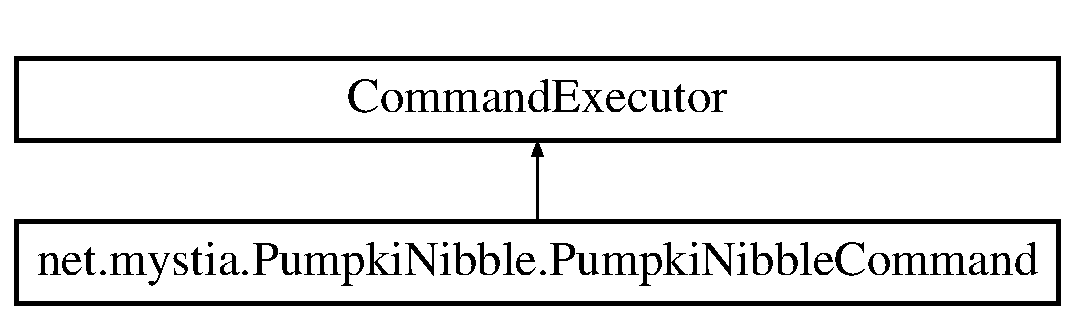
\includegraphics[height=2.000000cm]{classnet_1_1mystia_1_1_pumpki_nibble_1_1_pumpki_nibble_command}
\end{center}
\end{figure}
\subsection*{Public Member Functions}
\begin{DoxyCompactItemize}
\item 
\hypertarget{classnet_1_1mystia_1_1_pumpki_nibble_1_1_pumpki_nibble_command_aa5f604bca73970450a56f0f0b2125a55}{{\bfseries Pumpki\-Nibble\-Command} (\hyperlink{classnet_1_1mystia_1_1_pumpki_nibble_1_1_pumpki_nibble_main}{Pumpki\-Nibble\-Main} plugin)}\label{classnet_1_1mystia_1_1_pumpki_nibble_1_1_pumpki_nibble_command_aa5f604bca73970450a56f0f0b2125a55}

\item 
\hypertarget{classnet_1_1mystia_1_1_pumpki_nibble_1_1_pumpki_nibble_command_aee6de0c53289a26af562d3a80ea7f9be}{boolean {\bfseries on\-Command} (Command\-Sender sender, Command cmd, String label, String\mbox{[}$\,$\mbox{]} args)}\label{classnet_1_1mystia_1_1_pumpki_nibble_1_1_pumpki_nibble_command_aee6de0c53289a26af562d3a80ea7f9be}

\end{DoxyCompactItemize}


The documentation for this class was generated from the following file\-:\begin{DoxyCompactItemize}
\item 
src/main/java/net/mystia/\-Pumpki\-Nibble/Pumpki\-Nibble\-Command.\-java\end{DoxyCompactItemize}

\hypertarget{classnet_1_1mystia_1_1_pumpki_nibble_1_1_pumpki_nibble_listener}{\section{net.\-mystia.\-Pumpki\-Nibble.\-Pumpki\-Nibble\-Listener Class Reference}
\label{classnet_1_1mystia_1_1_pumpki_nibble_1_1_pumpki_nibble_listener}\index{net.\-mystia.\-Pumpki\-Nibble.\-Pumpki\-Nibble\-Listener@{net.\-mystia.\-Pumpki\-Nibble.\-Pumpki\-Nibble\-Listener}}
}
Inheritance diagram for net.\-mystia.\-Pumpki\-Nibble.\-Pumpki\-Nibble\-Listener\-:\begin{figure}[H]
\begin{center}
\leavevmode
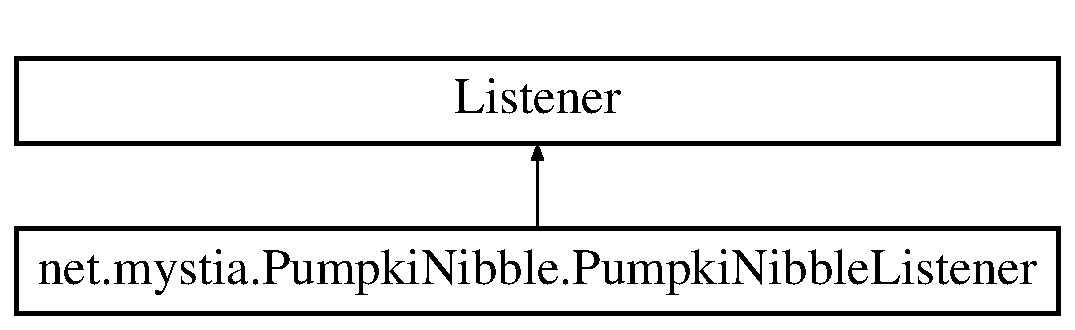
\includegraphics[height=2.000000cm]{classnet_1_1mystia_1_1_pumpki_nibble_1_1_pumpki_nibble_listener}
\end{center}
\end{figure}
\subsection*{Public Member Functions}
\begin{DoxyCompactItemize}
\item 
\hypertarget{classnet_1_1mystia_1_1_pumpki_nibble_1_1_pumpki_nibble_listener_ad3904862bb0646774ff82f8eea0da887}{void {\bfseries on\-Player\-Click} (Player\-Interact\-Event event)}\label{classnet_1_1mystia_1_1_pumpki_nibble_1_1_pumpki_nibble_listener_ad3904862bb0646774ff82f8eea0da887}

\end{DoxyCompactItemize}


The documentation for this class was generated from the following file\-:\begin{DoxyCompactItemize}
\item 
src/main/java/net/mystia/\-Pumpki\-Nibble/Pumpki\-Nibble\-Listener.\-java\end{DoxyCompactItemize}

\hypertarget{classnet_1_1mystia_1_1_pumpki_nibble_1_1_pumpki_nibble_main}{\section{net.\-mystia.\-Pumpki\-Nibble.\-Pumpki\-Nibble\-Main Class Reference}
\label{classnet_1_1mystia_1_1_pumpki_nibble_1_1_pumpki_nibble_main}\index{net.\-mystia.\-Pumpki\-Nibble.\-Pumpki\-Nibble\-Main@{net.\-mystia.\-Pumpki\-Nibble.\-Pumpki\-Nibble\-Main}}
}
Inheritance diagram for net.\-mystia.\-Pumpki\-Nibble.\-Pumpki\-Nibble\-Main\-:\begin{figure}[H]
\begin{center}
\leavevmode
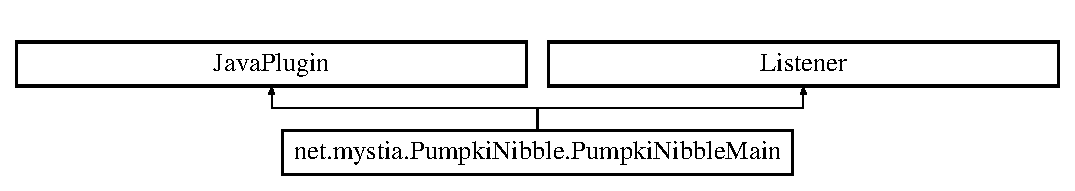
\includegraphics[height=2.000000cm]{classnet_1_1mystia_1_1_pumpki_nibble_1_1_pumpki_nibble_main}
\end{center}
\end{figure}
\subsection*{Public Member Functions}
\begin{DoxyCompactItemize}
\item 
\hypertarget{classnet_1_1mystia_1_1_pumpki_nibble_1_1_pumpki_nibble_main_a017f6f9ee132aa845d6f9835164b2be2}{void {\bfseries on\-Enable} ()}\label{classnet_1_1mystia_1_1_pumpki_nibble_1_1_pumpki_nibble_main_a017f6f9ee132aa845d6f9835164b2be2}

\item 
\hypertarget{classnet_1_1mystia_1_1_pumpki_nibble_1_1_pumpki_nibble_main_a7cb691f8f50867a245155243ad6aaf01}{void {\bfseries on\-Disable} ()}\label{classnet_1_1mystia_1_1_pumpki_nibble_1_1_pumpki_nibble_main_a7cb691f8f50867a245155243ad6aaf01}

\end{DoxyCompactItemize}
\subsection*{Static Public Attributes}
\begin{DoxyCompactItemize}
\item 
\hypertarget{classnet_1_1mystia_1_1_pumpki_nibble_1_1_pumpki_nibble_main_a7c44f28895a886f1155310b2e2839bc4}{static \hyperlink{classnet_1_1mystia_1_1_pumpki_nibble_1_1_pumpki_nibble_main}{Pumpki\-Nibble\-Main} {\bfseries p}}\label{classnet_1_1mystia_1_1_pumpki_nibble_1_1_pumpki_nibble_main_a7c44f28895a886f1155310b2e2839bc4}

\end{DoxyCompactItemize}


\subsection{Detailed Description}
Pumpki\-Nibble Plugin for Bukkit Allows users to eat Pumpkin\-Seeds and more!

Main class \begin{DoxyAuthor}{Author}
ron975 
\end{DoxyAuthor}


The documentation for this class was generated from the following file\-:\begin{DoxyCompactItemize}
\item 
src/main/java/net/mystia/\-Pumpki\-Nibble/Pumpki\-Nibble\-Main.\-java\end{DoxyCompactItemize}

\addcontentsline{toc}{part}{Index}
\printindex
\end{document}
